\chapter{Conclusion}

A collection of algorithms was presented which make creating an drawing for a mobile autonomous drawing robot an easy task. While no real world tests have yet been performed with the generated trajectories, comparing the results of the algorithm to the manually created drawings shows that the quality of the path is very much comparable, and the manual created drawings have been tested under real world conditions on a beach at the north sea.

\section{Outlook}
Of course, the problem is not solved to perfection yet. Several things can be improved and ideas are presented in the following section:

\paragraph{Driving over filled areas} The trackmarks are a serious problem for the drawing. While the connection paths can be manually adjusted to not cross through any already filled area, this is tedious and should be automatized. Different possible solutions would be:
\begin{itemize}
\item After an initial run of the TSP algorithm, the solution is examined. If a filled area is crossed over, that specific edge in the distance matrix is assigned a high weight, whereby the connection should not be included when the TSP is solved again. This process is repeated until a solution is found which minimizes the crossings of areas.
\item The intersections of the curved connection paths with already filled areas can easily be found by looking at the convex hulls of the Beziér curve control points that make up the connecting curve (a property of the Beziér curves is that they are always enclosed in the convex hull of the control points). 

If an intersection is evident, the polygon should get an offset which can be calculated by building the Minkowski sum of the polygon and a disk shape of some specified radius.  The offset polygon would be cutted and the appropriate part of that polygon would be added to the curve trajectory (as shown in \autoref{fig:super_conn}).
\item Another possibilty would be to add more $G^2$ spiro control points along the offset polygon which would have to maintain the same minimum distance to each other as defined in the section about smooth connection lines.
\end{itemize}

\begin{figure}
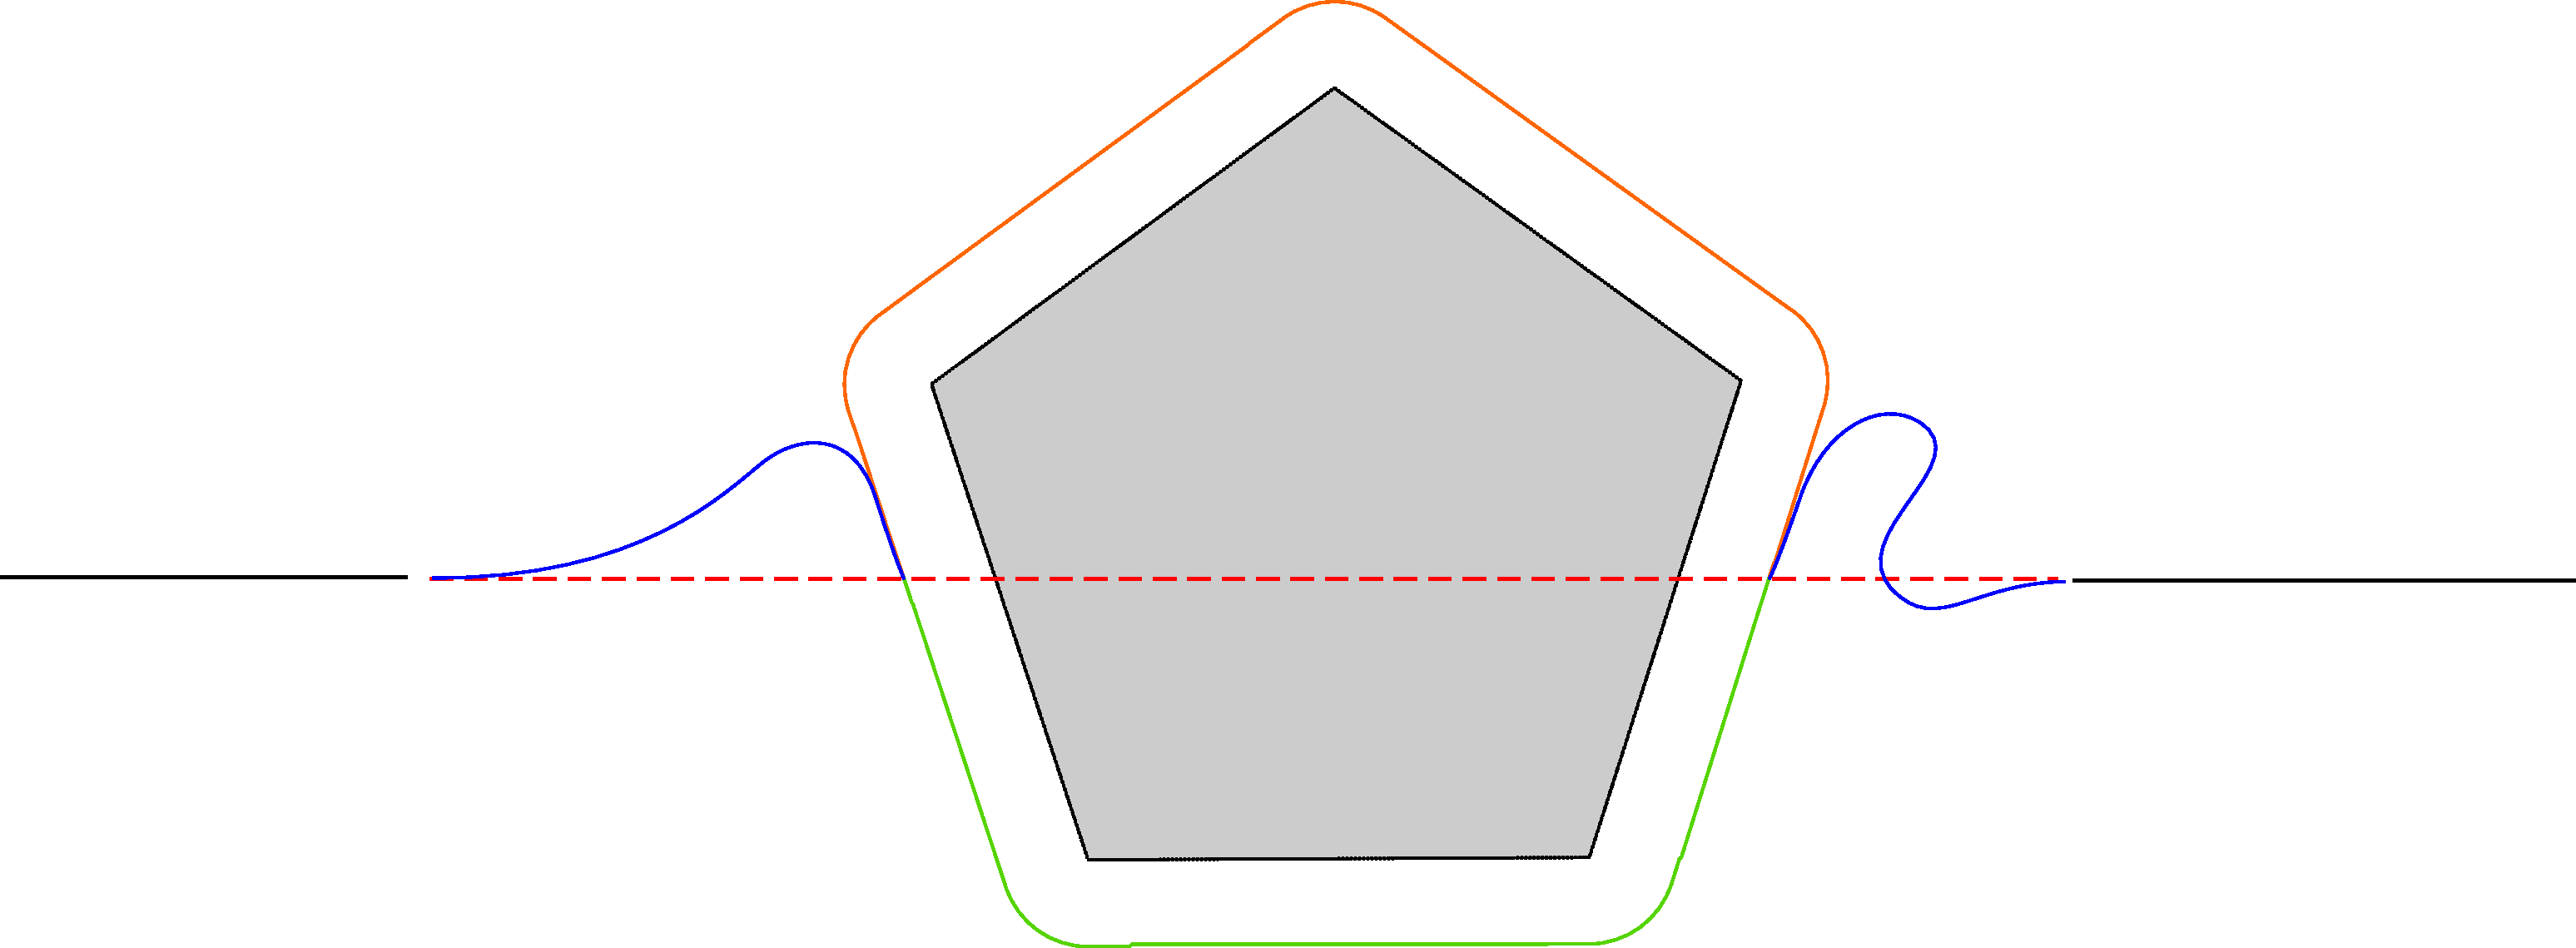
\includegraphics[width=\textwidth]{images/conclusion/minkowski_crossing_avoidance.pdf}
\caption{Using the Minkowski sum to offset the polygon and drive around the filled area (gray). The simple, straight connection is shown in red, the blue connection is the optimized, non-crossing connection.}
\end{figure}

\paragraph{Interactive Editing of Spiro Control Points} At the moment, the transition curve between two elements can only be edited in its Beziér representation. Because the Beziér representation of the curve consists of many more points, editing is more of difficult then editing the spiro control points (from which there are zero or two per curve). The user interface should include a way to move and add spiro control points. But the control points should keep the distance constraints described in \autoref{sec:smoothspiro}.

\paragraph{Missing Features in the User Interface} Some features are still missing from the user interface due to a lack of time: 

\begin{itemize}
\item Modifying global options such as the rounding radius or the line distance for the Zig Zag fill. These options are currently set per session and read from a configuration file. To change them, the server program has to be restarted.
\item Export and integration with path converter.
\item Post processing is not yet integrated into the user interface
\item The modified transition curves are not sent back to the server
\end{itemize}

All of the improvements are rather minor, but required for a fully functional system.